\documentclass[../../doc.tex]{subfiles}
\graphicspath{{\subfix{../../img}}}
\begin{document}
    \subsection{Обход препятствия}
    \begin{remark}
        Учёт фазовых ограничений в интегральной части функционала качества $J$, представленный в работе,
        позволяет лишь приближенно уписать условия вида
        $$
            g_i(x) \leqslant 0,
        $$
        которые часто встречаются в задачах, например, для обхода препятствия.
        Для этого функция $q$ выбирается таким образом, чтобы штрафовать за приближение траектории к препятствию.
        Для строго формального решения задачи с подобным условием,
        необходимо пользоваться методами расширенного лангранжиана~\cite{birgin2009},
        которые предполагают решение серии задач типа~\eqref{eq:kinematic}-\eqref{eq:cauchy}-\eqref{eq:continuos-cost}.
        Это приводит к существенному ухудшению асимптотики алгоритмов и тем самым увеличению времени работы программного решения.
    \end{remark}
    Пусть задано некоторое точечное препятствие с центром $e^{\textnormal{obstacle}}$ и радиусом $r^{\textnormal{obstacle}}$.
    Тогда зададим функцию цены:
    \begin{equation*}
        q(x) = \left| \left\| e^3(x) - e^{\textnormal{obstacle}} \right\|^2 - r^{\textnormal{obstacle}} \right|^{-2}
    \end{equation*}

    \begin{figure}[h]
        \begin{center}
            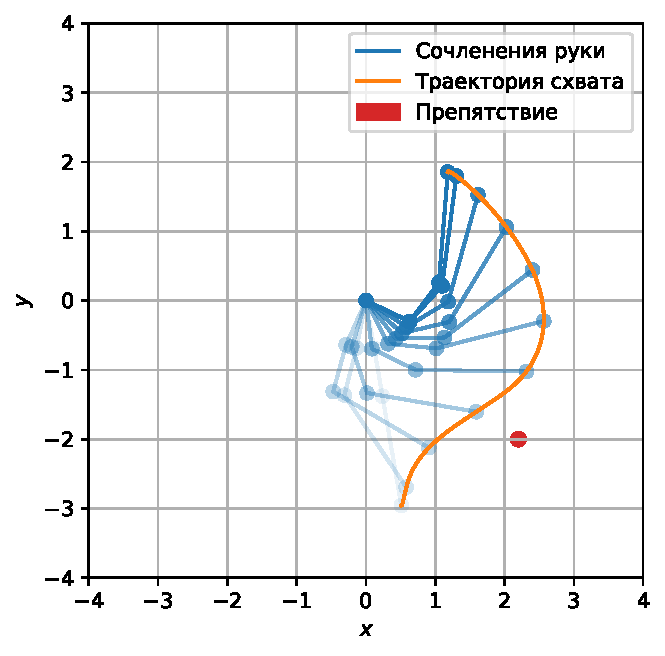
\includegraphics[width=0.49\textwidth]{examples/obstacle_pendulum}
            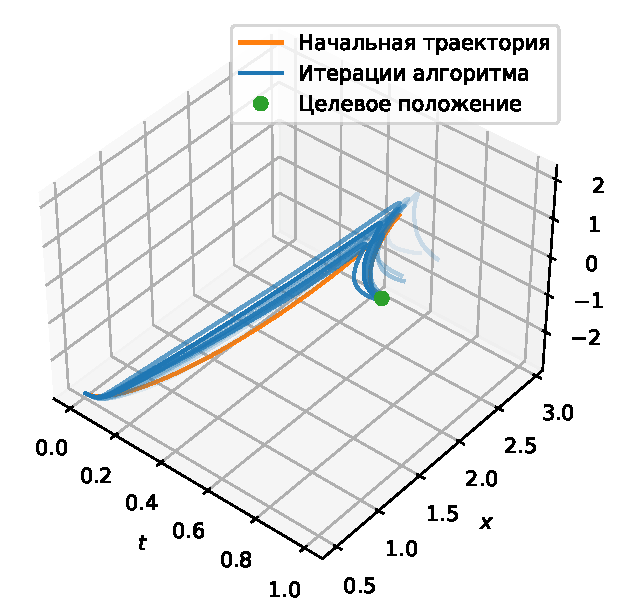
\includegraphics[width=0.49\textwidth]{examples/obstacle_endpoint}
        \end{center}
        \caption{Obstacle Task.}
    \end{figure}
    \begin{figure}[h]
        \begin{center}
            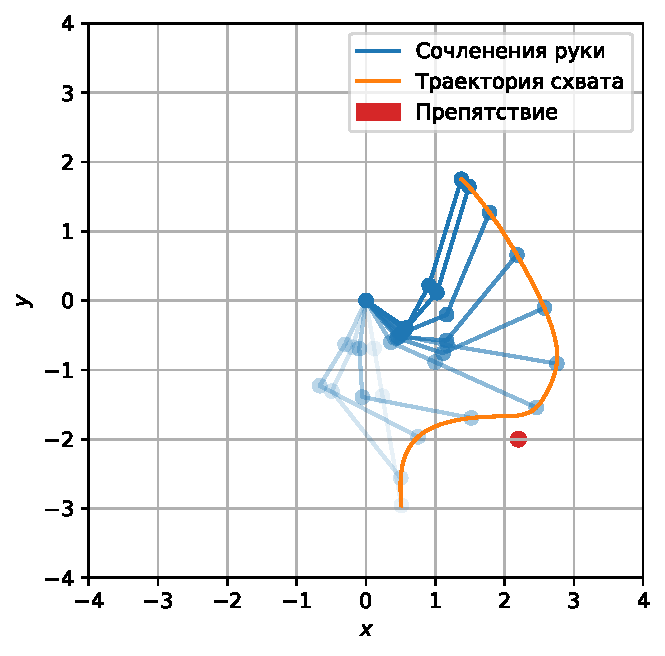
\includegraphics[width=0.49\textwidth]{examples/obstacle_pendulum_less}
            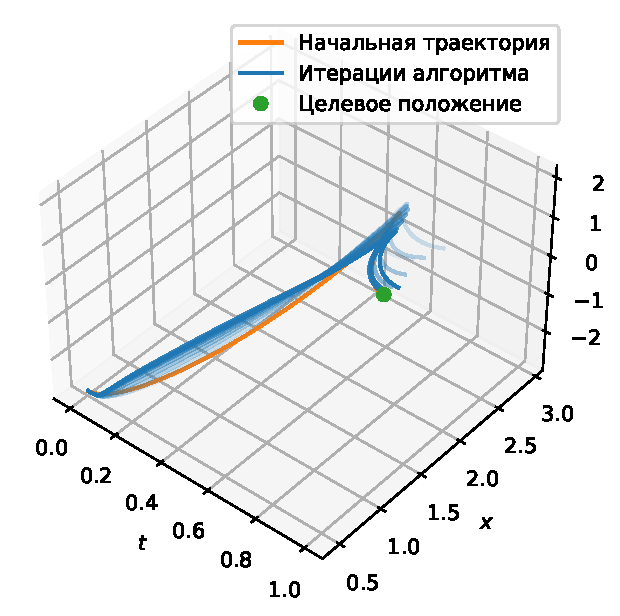
\includegraphics[width=0.49\textwidth]{examples/obstacle_endpoint_less}
        \end{center}
        \caption{Obstacle Less Task.}
    \end{figure}

    \ifSubfilesClassLoaded{
        \nocite{*}
        \clearpage
        \bibliographystyle{plain}
        \bibliography{../../refs}
    }{}
\end{document}